\documentclass{beamer}[10]
% preamble speciale Jacob Harder
% 31. jan. 2020

%packages

\usepackage[utf8]{inputenc} %utf8 is probably good
\usepackage{amsmath}
\usepackage{amssymb}
\usepackage{amsthm}
\usepackage{graphicx} %for including images
\usepackage{float} %for exact placement of figure (and more?)
\usepackage{mathtools} %for \mathclap (stacking under sums)
\usepackage{dsfont} %for boldface numbers
\usepackage{bm} %vectors in bold
\usepackage[ruled,vlined]{algorithm2e}
\usepackage{cleveref}
\usepackage{ifthen}
\usepackage{commath}
\usepackage[a4paper,width=150mm,top=25mm,bottom=25mm]{geometry}
\usepackage{upgreek}
%\usepackage[inline]{enumitem}
\usepackage{multicol}
%\usepackage{fancyhdr} %maybe later..
%\pagestyle{fancy}
\usepackage{mathabx}
\usepackage{csquotes}
\usepackage{tikz}
\usepackage{outline} %for subitems in lists

%front page
\usepackage{wallpaper}
\usepackage{titling}

%bibliography
\usepackage[numbers]{natbib}
\bibliographystyle{plainnat}
\newcommand{\mcite}[1]{[\citenum{#1}, \citeauthor{#1} (\citeyear{#1})]}
\newcommand{\ncite}[1]{\cite{#1}}

%linespread and geometry
\linespread{1.3}

%commands
\newcommand{\Cal}{\mathcal}
\newcommand{\cl}{\mathcal}
\newcommand{\fk}{\mathfrak}
\newcommand{\bb}{\mathbb}
\newcommand{\Q}{\bb{Q}}
\newcommand{\Z}{\bb{Z}}
\newcommand{\N}{\bb{N}}
\newcommand{\R}{\bb{R}}
\newcommand{\C}{\bb{C}}
\newcommand{\E}{\bb{E}}
\newcommand{\Rext}{\ol{\ul{\R}}}
\newcommand{\Var}{\mathrm{Var}}
\newcommand{\Prob}{\mathds{P}} %fundamental probability measure
\newcommand{\idc}{\mathds{1}}
\newcommand{\ve}{\varepsilon} %abbreviation for epsilon
\newcommand{\Yp}{\Upupsilon} %abbreviation for Ypsilon
\newcommand{\difd}{\; \mathrm{d}} %differential d
\newcommand{\wt}{\widetilde}
\newcommand{\wh}{\widehat}
\newcommand{\ol}{\overline}
\newcommand{\ul}{\underline}
\newcommand{\Mid}{\;\middle\vert\;}
\newcommand{\id}{\text{id}}
\newcommand{\supp}{\text{supp}}
\newcommand{\defemph}[1]{\textbf{#1}} %first-mentions of names
\DeclarePairedDelimiter\ceil{\lceil}{\rceil}
\DeclarePairedDelimiter\floor{\lfloor}{\rfloor}
\DeclareMathOperator*{\argmax}{argmax}
\DeclareMathOperator*{\argmin}{argmin}
\newcommand{\defeq}{\vcentcolon=} %definition equality symbol
%add single eq. tag in align*
\newcommand\numberthis{\addtocounter{equation}{1}\tag{\theequation}}
\newcommand{\rleft}[1]{\rotatebox[origin=c]{90}{\ensuremath{#1}}}
\newcommand{\vrel}[3]{ % for vertical subseteq e.g.
\vcenter{\halign{\hfill##\hfill\cr
\ensuremath{#1}\cr
\rotatebox[origin=c]{270}{\ensuremath{#2}}\cr
\ensuremath{#3}\cr
}}}
\newcommand{\lar}{\leftrightarrow}
\newcommand{\Span}{\mathrm{span}}
\newcommand{\Gr}{\mathrm{Gr}}

%theorems
\theoremstyle{definition}
\newtheorem{thm}{Theorem}[chapter]
\newtheorem{lem}[thm]{Lemma}
\newtheorem{defn}[thm]{Definition}
\newtheorem{cor}[thm]{Corollary}
\newtheorem{rem}[thm]{Remark}
\newtheorem{prop}[thm]{Proposition}
\newtheorem{asm}{Assumption}
\newtheorem{example}[thm]{Example}
%\newtheorem{cond}{Condition}
\newtheorem{sett}{Setting}
\newtheorem{innercond}{Condition}
\newenvironment{cond}[1]
  {\renewcommand\theinnercond{#1}\innercond}
  {\endinnercond}

%cref
\crefname{algocf}{alg.}{algs.}
\Crefname{algocf}{Algorithm}{Algorithms}
\crefname{innercond}{}{}
\Crefname{innercond}{}{}


\usepackage{pgf}
%\usepackage[danish]{babel}
\usepackage[utf8]{inputenc}
\usepackage{beamerthemesplit}
\usepackage{graphics,epsfig, subfigure}
\usepackage{url}
\usepackage{srcltx}
\usepackage{hyperref}
\usepackage{tikz-dependency}
\usepackage{tikz-qtree}
\usepackage{wrapfig}
\usepackage{algorithm2e}
\usepackage{algorithmic}

\definecolor{kugreen}{RGB}{50,93,61}
\definecolor{kugreenlys}{RGB}{132,158,139}
\definecolor{kugreenlyslys}{RGB}{173,190,177}
\definecolor{kugreenlyslyslys}{RGB}{214,223,216}
\setbeamercovered{transparent}
\mode<presentation>
\usetheme[
  width=1.6cm,
  numbers,
  totalnumber,
  compress,
  sidebarshades,
  hideothersubsections
]{PaloAlto}
\setbeamertemplate{footline}[frame number]

\usecolortheme[named=kugreen]{structure}
\useinnertheme{circles}
\usefonttheme[onlymath]{serif}
\setbeamercovered{transparent}
\setbeamertemplate{blocks}[rounded][shadow=true]

\logo{\includegraphics[width=0.5cm]{KULogo}}

\makeatletter
\beamer@headheight=1.5\baselineskip     %controls the height of the headline, default is 2.5
\makeatother

\title{Theoretical aspects of Q-learning}
\subtitle{Masters thesis defense}
\institute{Jacob Harder \\
Department of Mathematical Sciences \\ University of Copenhagen}
\date{26 June, 2020}

\begin{document}

\frame{\titlepage \vspace{-0.5cm}
}

\frame
{
\frametitle{Overview}
\tableofcontents%[pausesection]
}

\section{Introduction}

\begin{frame}
  \frametitle{Q-learning as AI}
  \usetikzlibrary{trees, arrows, shapes.multipart}
  \tikzset{
    edge from parent/.style={draw,-latex},
    level distance=1.5cm
  }
  \begin{tikzpicture}[
      every node/.style={align=center,anchor=north},
    ]
    \Tree [.{Artificial Intelligence (AI)}
      [.{Machine Learning (ML)}
	[.{Reinforcement Learning (RL)}
	  [.{\defemph{Q-learning}} ]
	]
	[.{Supervised Learning, etc.} ]
      ]
    ]
  \end{tikzpicture}
\end{frame}

\frame{
  \frametitle{Machine learning}
  Machine Learning is
  ``the study of computer algorithms that improve automatically through
  \emph{experience}''.
  \begingroup
  \fontsize{10pt}{12pt}\selectfont
  \begin{itemize}
    \item[-] \defemph{Supervised learning}: Tasks are learned from data 
      based on feedback from a
      \emph{supervisor}. E.g. image classification.
    \item[-] \defemph{Unsupervised learning}:
      Data is given without evaluatory feedback,
      general trends about the data are analysed.
      E.g. principal component analysis, and cluster analysis.
    \item[-] $\rightarrow$\footnote{``$\rightarrow$'': Our main area of focus
      in this thesis.}
	\defemph{Reinforcement learning}: Algorithms
      which learns through interactions with an \emph{environment}.
  \end{itemize}
  \endgroup
}

\frame{
  \frametitle{Challenges in RL}
  Challenges in Reinforcement Learning include:
  \begingroup
  \fontsize{10pt}{12pt}\selectfont
  \begin{itemize}
    \item[-] \defemph{Exploration-exploitation trade-off}. Training and
      performing occurs simultaneously so one optimizes the total reward on some
      time horizon. This is studied
      in e.g. the multi-armed bandit problem.
    \item[-] $\rightarrow$ \defemph{Deriving optimal policies}.
      Training and performing is
      distinguished and emphasis is put on the expected performance of the final
      derived policy rather than rewards occuring during training.
  \end{itemize}
  \endgroup
}

\subsection{The environment}

\frame{
  \frametitle{The environment}
  The \defemph{environment} in RL is often formalized as a
  \defemph{Markov decision process} (MDP), which consists of
  \begin{itemize}
    \item[-] $\Cal{S}$ a 
      measurable space of states.
    \item[-] $\Cal{A}$ a 
      measurable space of actions.
    \item[-] $P : \Cal{S} \times \Cal{A} \leadsto \Cal{S}$
      a transition kernel\footnote{
	Here $\leadsto$ denotes a \emph{stochastic mapping} (to be
      defined soon).}.
    \item[-] $R : \Cal{S} \times \Cal{A} \leadsto \R$
      a reward kernel discounted by
    \item[-] a discount factor $\gamma \in [0,1)$.
    \item[-] $\frak{A}(s) \subseteq \cl{A}$ a set of admissable actions
      for each $s \in \cl{S}$.
  \end{itemize}
}

\frame{
  \frametitle{Examples of MDPs}
  Examples of Markov decision processes include
  \begin{itemize}
    \item[-] Board games where one plays against a fixed opponent,
      e.g. \emph{chess} where the set of states $\cl{S}$
      is the set of all obtainable chess-positions.
    \item[-] Time-descretized physics simulations with action inputs and reward
      outputs, including most single player video games and
      the classic \emph{cartpole} example (balancing a stick).
  \end{itemize}
}

\frame{
  \begingroup
  \fontsize{10pt}{12pt}\selectfont
  \frametitle{The probability kernels}
  \begin{block}{Probability kernel}
    A \defemph{probability kernel}
    (also called a \emph{stochastic mapping}, \emph{stochastic kernel}
    or \emph{Markov kernel})
    $\kappa : \cl{X} \leadsto \cl{Y}$ is a collection of probability measures
    $\kappa(\cdot \mid x)$, one for each $x \in \cl{X}$ such that
    for any measurable set $B \subseteq \cl{Y}$ the function
    $x \mapsto \kappa(B \mid x)$ is measurable.
  \end{block}
  The transition probability measure $P(\cdot \mid s, a)$ 
  of the pair $(s, a) \in \cl{S} \times \cl{A}$ determines
  what states are likely to follow after \emph{being} in state $s$ and
  \emph{choosing} action $a$. Similarly from the reward kernel $R$ one obtains the
  measure $R(\cdot \mid s, a)$ determining the reward distribution following
  the timestep $(s, a)$.
  \endgroup
}

\frame{
  \frametitle{Policies}
  Given a Markov decision process one can define a \defemph{policy} $\pi$ by
  sequence of probability kernels $\pi = (\pi_1, \pi_2, \dots)$ where
  $\pi_i : \cl{H}_i \leadsto \cl{A}$ and
  $\cl{H}_i = \cl{S} \times \cl{A} \times \dots \times \cl{S}$
  is the \emph{history space} at the $i$th timestep.
}

\frame{
  \frametitle{Stochastic processes}
  An MDP $(\cl{S}, \cl{A}, P, R, \gamma)$ together with a policy
  $\pi = (\pi_1, \pi_2, \dots)$ and a distribution $\mu$ on $\cl{S}$
  give rise to a stochastic process
  $(S_1, A_1, S_2, A_2, \dots) \sim \kappa_\pi \mu$ such that for any
  $i \in \N$ we have
  $(S_1, A_1, \dots, S_i) \sim P\pi_{i-1} \dots P \pi_1 \mu$
  where $P\pi_{i-1} \dots P \pi_1$ denotes the \emph{kernel-composition}
  of the probability kernels $P, \pi_1, \dots, \pi_{i-1}$.
  We denote by $\E_s^\pi$ expectation over $\kappa_\pi \mu$ where
  $\mu = \delta_s$, that is, $S_1 = s$ a.s.
}

\subsection{Value functions and the goal of RL}

\frame{
  \frametitle{Policy evaluation}
  For a policy $\pi$ we can define the policy evaluation function:
  \begin{block}{Policy evaluation}
    \begingroup
    \small
    Denote by $r(s, a) = \int x \difd R(x \mid s, a)$ the \emph{expected
    reward function}. We define the \defemph{policy evaluation function} by
    $$ V_\pi(s) = \E_s^\pi \sum_{i=1}^\infty \gamma^{i-1} r \circ \rho_i $$
    where $\rho_i$ is projection onto $(\cl{S}_i, \cl{A}_i)$.
    \endgroup
  \end{block}
  This an example of a (state-) \emph{value function}, as it assigns a real
  number to every state $s \in \cl{S}$.
}

\frame{
  \frametitle{Finite policy evaluation}
  Similar to the infinite horizon policy evaluation we can also consider
  a finite horizon version:
  \begin{block}{Definition: Finite policy evaluation}
    We define the function $V_{n, \pi} : \cl{S} \to \R$ by
    \[ V_{n,\pi}(s) = \E_{s}^\pi \sum_{i=1}^n \gamma^{i-1} r \circ \rho_i \]
    called the $k$th \defemph{finite policy evaluation}\footnote{When
    $n=0$ we say $V_{0,\pi} = V_0 \defeq 0$ for any $\pi$.}.
  \end{block}
}

\frame{
  \frametitle{Optimal value function}
  \begingroup
  \footnotesize
  \begin{block}{Definition: Optimal value functions}
    \begin{align*}
      V_n^*(s) \defeq & \; \sup_{\pi \in R\Pi} V_{n,\pi}(s)
      = \sup_{\pi \in R\Pi} \E_s^\pi \sum_{i=1}^n r_i
      \\
      V^*(s) \defeq & \; \sup_{\pi \in R\Pi} V_\pi(s)
      = \sup_{\pi \in R\Pi} \E_s^\pi \sum_{i=1}^\infty r_i
    \end{align*}
    This is called the \defemph{optimal value function} (and the $n$th
    optimal value function).
    A policy $\pi^* \in R\Pi$ for which $V_{\pi^*} = V^*$ is called an
    \defemph{optimal policy}.
    If $V_{n, \pi^*} = V^*_n$ then $\pi^*$ is called $n$-optimal.
  \end{block}
  Provided such an optimal policy $\pi^*$ exists,
  obtaining such a policy is the ultimate goal
  of Reinforcement Learning.
  \endgroup
}

\subsection{Value iteration}

\frame{
  \frametitle{Greediness}
  In order to show existence of optimal policies and talk about algorithms
  which can determine such policies, we define the concept of \emph{greediness}.
}

\frame{
  \frametitle{Greedy actions}
  \begingroup
  \footnotesize
  The purpose of (most) value functions $V : \cl{S} \to \R$ is to give an estimate
  on how \emph{good} a certain state is, in terms of the rewards one may expect
  after visiting it.
  \\ This give rise to the idea of \emph{greedy actions}, that is,
  actions leading to states high \emph{values} (according to $V$).
  \begin{block}{Definition greedy actions}
    Let $V : \cl{S} \to \R$ be a measurable value-function.
    We define
    \[ G_V(s) = \argmax_{a \in \frak{A}(s)} T_a V(s) \subseteq \frak{A}(s) \]
    as the set of \defemph{greedy} actions w.r.t. $V$.
  \end{block}
  \endgroup
}

\frame{
  \frametitle{Greedy policies}
  Greedy actions leads to \emph{greedy policies}:
  \begin{block}{Definition: Greedy policy}
    Let $V : \cl{S} \to \R$ be a measurable value-function and
    let $\tau : \cl{S} \leadsto \cl{A} \in S\Pi$ be a stationary policy.
    If there exists a measurable $G_V^\tau(s) \subseteq G_V(s)$
    such that
    \[ \tau(G_V^\tau(s) \mid s) = 1 \]
    for every $s \in \cl{S}$, then $\tau$ is called greedy w.r.t. $V$.
    We will often denote a $V$-greedy policy by $\tau_V$.
  \end{block}
}

\frame{
  \frametitle{Existence of greedy policies}
  \begingroup
  \footnotesize
  \begin{block}{Theorem (Existence of greedy policies)}
    Suppose $V: \cl{S} \to \R$ is \emph{upper semicontinuous} and that
    \begin{itemize}
      \item[1.] $\cl{S}$ and $\cl{A}$ are standard Borel.
      \item[2.]  The set of admissable actions 
	$\frak{A}(s) \subseteq \cl{A}$ is compact for all $s \in \cl{S}$
	and $\Gamma = \{ (s, a) \in \cl{S} \times \cl{A} \mid a \in \frak{A}(s) \}$
	is a closed subset of $\cl{S} \times \cl{A}$.
      \item[3.] The transition kernel $P$ is continuous.
      \item[4.] The expected reward function $r = \int r' \difd R(r' \mid \cdot)$
	is upper semicontinuous and bounded from above.
    \end{itemize}
    Then there exists a deterministic policy $\pi_V$ which is greedy for $V$.
  \end{block}
  If assumptions 1.-4. hold we will say that the MDP is \emph{greedy}.
  \endgroup
}

\frame{
  \frametitle{Policy iteration}
  \begingroup
  \footnotesize
  Using the concepts we have defined one can get the following idea:
  Iteratively generate value functions by
  picking greedy policies and then evaluating these policies.
  This is called \emph{policy iteration}.
  \begin{figure}
    \centering
    \begin{tikzpicture}
      \def \n {3}
      \def \radius {1cm}
      \def \margin {30} % margin in angles, depends on the radius
      \def \txt {
	{$V$},
	{$\tau_V$},
	{$V_{\tau_V}$}
      }

      \foreach \t [count=\s from 0] in \txt
      {
	\node[draw, circle] at ({360/\n * (\s - 1)}:\radius) {\t};
	\draw[->, >=latex] ({360/\n * (\s - 1)+\margin}:\radius)
	arc ({360/\n * (\s - 1)+\margin}:{360/\n * (\s)-\margin}:\radius);
      }
    \end{tikzpicture}
  \end{figure}
  Policy iteration is a well studied algorithm and can be shown to
  converges to optimum for a variety of environments. We will however
  move on to talk about a related concept called
  \emph{value iteration}.
  \endgroup
}

\frame{
  \frametitle{Operators on value functions}
  Before defining value iteration we introduce some operators
  \begin{block}{The $T$-operators}
    For a stationary policy $\tau \in S\Pi$ and a value function
    $V:\Cal{S} \to \R \in \cl{L}_\infty(\cl{S})$
    we define the operators 
    \begin{gather*}
      \text{The policy evaluation operator: }
      \\ T_\tau V \defeq s \mapsto \int r(s, a)
      + \gamma V(s') \difd (P \tau)(a, s'\mid s)
      \\ \text{The Bellman optimality operator: }
      \\ T V \defeq s \mapsto 
      \sup_{a \in \frak{A}(s)} \left(r(s, a) + \gamma \int V(s')
      \difd P(s' \mid s, a) \right)
    \end{gather*}
  \end{block}
}

\frame{
  \frametitle{Properties of the $T$-operators}
  \begingroup
  \footnotesize
  \begin{block}{Proposition (Properties of the $T$-operators)}
    \begin{itemize}
      \item $V_{k, \pi} = T_{\tau_1} V_{k-1, (\tau_2, \dots)}
	= T_{\tau_1} \dots T_{\tau_k} V_0$.
      \item $V_\pi = \lim_{k \to \infty} T_{\tau_1} \dots T_{\tau_k} V_0$
      \item For the stationary policy $\tau$ we have $T_\tau V_\tau = V_\tau$.
      \item $T$ and $T_\tau$ are $\gamma$-contractive
	on $\Cal{L}_\infty(\Cal{S})$.
      \item $V_\tau$ is the unique bounded fixed point of $T_\tau$
	in $\Cal{L}_\infty(\Cal{S})$.
    \end{itemize}
  \end{block}
  This way $T_\tau$ can be interpreted as a 'one-step policy evaluation, when
  following the policy $\tau$'.
  On the other hand $T$ can be interpreted as a 'one-step evaluation, when
  always choosing greedy actions'.
  \endgroup
}

\frame{
  \frametitle{Value iteration}
  \begingroup
  \footnotesize
  \emph{Value iteration} is the iterative application of the $T$-operator.
  The following theorem show why
  value iteration is a 
  central idea Reinforcement Learning\footnote{Actually value iteration
  is inherited from dynamic programming.}.
  \begin{block}{Theorem (Existence optimal policies
    \& convergence of value iteration)}
    Given a greedy MDP we have that
    \[ V^*_k = T^k V_0 = T_{\tau^*_{k-1}} \dots T_{\tau^*_0} V_0
    = V_{k, (\tau^*_{k-1}, \dots, \tau^*_0)} \]
    The policy $(\tau^*_{k-1}, \dots, \tau^*_0)$ is a deterministic
    $k$-optimal policy
    where $\tau_k^* = \tau_{T^k V_0}$ is any deterministic
    greedy policy for $T^k V_0$ for any $k \in \N$.
    \\ Furthermore $V^* = \lim_{k\to\infty} T^k V^*_0$, the greedy policy
    $\tau^* = \tau_{V^*}$ exists and an optimal policy.
  \end{block}
  \endgroup
}

\frame{
  \frametitle{Convergence rates}
  We can also show that the optimal value function $V^*$ is a fixed point of
  the Bellman optimality operator $T$.
  \[ TV^* = V^* \]
  This is often called \emph{Bellman's optimality equation}.
  \\ Recalling that $T$ is $\gamma$-contractive, by Banach's fixed point theorem 
  we get exponential convergence rates for value iteration:
  \[ \norm{T^k V - V^*} \leq \gamma^k \norm{V - V^*}_\infty = \cl{O}(\gamma^k) \]
}

\frame{
  \frametitle{Example: Gridworld}
  \begingroup
  \footnotesize
  \begin{wrapfigure}{R}{0.5\textwidth}
    \centering
    \begin{tikzpicture}
      \draw[step=0.5cm, color=gray] (0,0) grid (2.5,2.5);
      \node (A) at (0.75,2.25) {A};
      \node (A') at (0.75,0.25) {A'};
      \node (B) at (1.75,2.25) {B};
      \node (B') at (1.75,1.25) {B'};
      \draw [->][bend left=15] (A) edge node[left] {\scriptsize{+10}} (A');
      \draw [->][bend left=15] (B) edge node[left] {\scriptsize{+5}} (B');
    \end{tikzpicture}
  \end{wrapfigure}
  The \emph{gridworld} MDP consist of 25 states $\cl{S} = [5]^2$ and 4 actions
  $\cl{A} = \{U, D, L, R\}$ for \emph{up}, \emph{down}, \emph{left} and 
  \emph{right} and moves the agent
  1 square up, down, left or right.
  A reward of 0 is given by default, except when
  \begingroup
  \scriptsize
  \begin{itemize}
    \item[-] \emph{hitting the boundary} a reward of -1 is given
    \item[-] when in $A = (2,1)$ any action moves to $A' = (2,5)$ and
      is rewarded 10.
    \item[-] when in $B = (4,1)$ any action moves to $B' = (4,3)$ and
      is rewarded 5.
  \end{itemize}
  \endgroup
  Finally $\gamma = 0.9$ is the standard value of the discount factor
  in this example.
  \endgroup
}

\frame{
  \frametitle{Example: Gridworld}
  \begin{figure}
    \centering
    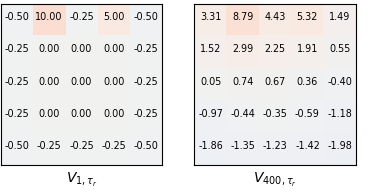
\includegraphics[scale=0.8]{figs/gridworld1_1.png}
    \caption{Policy evaluations of the gridworld environment.
      Note that $V_{\max} \cdot \gamma^{400} = 100 \cdot (0.9)^{400}
      \approx 4.97 \cdot 10^{-17}$ so $V_{\tau_r, 400}$
      are very close to the true infinite horizon value functions
    $V_{\tau_r}$ (providing numerical errors are insignificant).}
    \label{fig:gw1}
  \end{figure}
}

\frame{
  \frametitle{Example: Gridworld}
  \begin{figure}
    \centering
    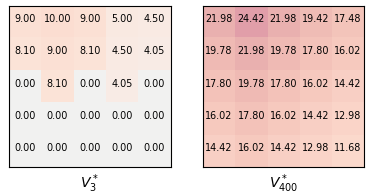
\includegraphics[scale=0.8]{figs/gridworld1_2.png}
    \caption{Optimal value functions of the gridworld environment.
      By the same upper bound as before we have
    $\norm{V^* - V^*_{400}}_\infty < 4.97 \cdot 10^{-17}$.}
    \label{fig:gw1}
  \end{figure}
}

\frame{
  \frametitle{Example: Gridworld}
  \vspace{-0.35cm}
  \begin{figure}
    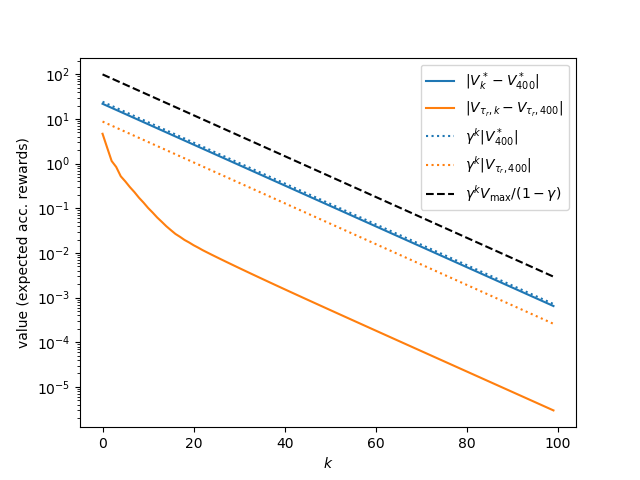
\includegraphics[scale=0.45]{figs/gridworld2.png}
  \end{figure}
  \footnotesize Convergence of gridworld value functions compared with
  the theoretical bounds. The black dashed line is the general theoretical
  bound for both $T$ and $T_{\tau}$ by Banachs fixed point theorem and
  the maximum value $V_{\max} = R_{\max} / (1-\gamma)$.
  The dotted blue and orange uses $\abs{V_k^*}$ and $\abs{V_{\tau, k}}$ 
  respectively, which might not be available.
  ($\gamma = 0.9$).
}

\subsection{Q-functions}

\frame{
  \frametitle{Q-functions}
  A \defemph{Q-function}
  is simply any function assigning a real number to every state-action pair.
  They are also called (state-) \emph{action value functions}.
  \\ \vspace{0.3cm}
  A \defemph{Q-learning} algorithm is any algorithm which uses Q-functions
  to derive a policy for an environment\footnote{Some authors refer to
    Q-learning as a specific variation of temporal difference learning,
    but this fails to capture many algorithms which are also referred to
  as \emph{Q-learning algorithms}.}.
}

\frame{
  \frametitle{Motivation for Q-functions}
  A clear advantage of working with Q-function
  $Q:\Cal{S}\times\Cal{A} \to \R$ rather than a value function
  $V:\Cal{S}\to \R$,
  is that finding the optimal action $a^* \in \frak{A}(s)$ at state $s$
  requires only a maximization over the Q-function itself:
  $a^* = \argmax_{a \in \frak{A}(s)} Q(s,a)$.
  This should be compared to finding an optimal action
  according to a value function $V$:
  $a^* = \argmax_{a \in \frak{A}(s)} r(s,a) + \gamma \E_{P(\cdot \mid s,a)} V$.
}

\frame{
  \frametitle{Greed with Q-functions}
  Formally we define greedy actions and policies w.r.t. a Q-function as
  \begingroup
  \small
    Let $Q:\cl{S} \times \cl{A} \to \R$ be a measurable Q-function and
    $\tau: \cl{S} \leadsto \cl{A}$ be a (stationary) policy.
  \begin{block}{Greedy policy}
    Define the set of
    \emph{greedy actions} by
    $G_Q(s) \defeq \argmax_{a \in \frak{A}(s)} Q(s, a)$.
    If there exist a measurable set $G_Q^\tau(s) \subseteq G_Q(s)$
    for every $s \in \Cal{S}$ such that
    \[ \tau \left( G_Q^\tau(s) \Mid s \right) = 1 \]
    then $\tau$ is said to be \defemph{greedy} with respect to $Q$ and is
    denoted $\tau_Q$.
  \end{block}
  \endgroup
}

\frame{
  \frametitle{Q-function operators}
  \begingroup
  \footnotesize
  Moreover we define $T$-operators similar to ones for value functions
  \begin{block}{Operators for Q-functions}
    For any stationary policy $\tau \in S\Pi$ and
    integrable Q-function $Q:\Cal{S} \times \Cal{A} \to \R
    \in \cl{L}_\infty(\cl{S} \times \cl{A})$ we define
    \begin{gather*}
      \text{Next-step operator: }
      \\ P_\tau Q(s, a) = \int Q(s', a') \difd \tau P(s', a' \mid s, a)
      \\ \text{Policy evaluation operator: } 
      \\
      T_\tau Q(s, a) = 
      r(s, a) + \gamma \int Q(s', a') \difd \tau P(s', a' \mid s, a)
      \\ \text{Bellman optimality operator: } 
      \\ T Q(s, a) = r(s, a) + \gamma
      \int \max_{a' \in \Cal{A}} Q(s', a') \difd P(s' \mid s, a)
    \end{gather*}
    where $T_a = T_{\delta_a}$.
  \end{block}
  \endgroup
}

\frame{
  \frametitle{Relation between value- and Q-functions}
  \begingroup
  \footnotesize
  \begin{block}{Theorem (Relations between Q- and value functions)}
    Let $\pi = (\tau_1, \tau_2, \dots) \in M\Pi$ be a Markov policy
    and $\tau \in S\Pi$ stationary. Then
    \begin{itemize}
      \item[-] Policy evaluations are related by
	$\E_{\tau(\cdot \mid s)} Q_{k, \pi} = V_{k+1, (\tau, \pi)}(s)$.
      \item[-] $T_\tau$-operators are related by $T_\tau Q_{k, \pi}(s, a)
	= r + \gamma \E_{P(\cdot \mid s, a)} T_\tau V_{k, \pi}$.
      \item[-] $\tau$ is greedy for
	$Q_{k, \pi}$ if and only if $\tau$ is greedy for $V_{k, \pi}$
	and
	\\ $\tau$ is greedy for $Q_\pi$ if and only if $\tau$ is greedy for
	$V_\pi$.
      \item[-] Optimal policies are related by
	$\max_{a \in \frak{A}(s)} Q^*(s, a) = V^*(s)$ and
	\[ Q^*_k(s, a) = r(s, a) + \gamma \E_{P(\cdot \mid s, a)} V^*_k,
	\quad Q^*(s, a) = r(s, a) + \gamma \E_{P(\cdot \mid s, a)} V^* \]
    \end{itemize}
  \end{block}
  \endgroup
}

\frame{
  \frametitle{Properties of Q-functions}
  Because of the close relations
  many properties are inherited from value function to Q-functions:
  \begin{block}{Proposition (Properties of Q-functions)}
    Let $\pi = (\tau_1, \tau_2, \dots) \in M\Pi$ be a Markov policy
    and $\tau \in S\Pi$ stationary. Then
    \begin{itemize}
      \item $Q_{k, \pi} = T_{\tau_1} \dots T_{\tau_k} Q_0$ and
	$Q^*_k = T^k Q^*_0$.
      \item $Q_\pi = \lim_{k \to \infty} Q_{k, \pi}$ and
	$Q^* = \lim_{k\to\infty} Q_k^*$. 
      \item $T,\; T_\tau$ are $\gamma$-contractive on
	$\Cal{L}_\infty(\Cal{S}\times\Cal{A})$
	and $Q^*,\; Q_\tau$ are their unique fixed points.
      \item $Q^* = Q_{\tau^*}$
    \end{itemize}
  \end{block}
}

\subsection{Q-iteration}

\begin{frame}[fragile]
  \frametitle{Q-iteration}
  \begingroup
  \small
  \emph{Q-iteration} is the analogue of value-iteration for Q-function.
  It can be stated in the form of an algorithm as follows:
  \begin{block}{Algorithm (Q-iteration)}
    \begin{algorithm*}[H]
      \KwData{MDP $(\cl{S}, \cl{A}, P, R, \gamma)$, number of iterations $K$}
      Initialize expected reward function
      $r \leftarrow \int x \difd R(x \mid \cdot)$
      and $\wt{Q}_0 \leftarrow r$.
      \\ \For{$k = 0,1, \dots K-1$}{
	$\wt{Q}_{k+1} \leftarrow T \wt{Q}_k$
      }
      \KwOut{$\wt{Q}_K$}
    \end{algorithm*}
  \end{block}
  In the context of a greedy MDP we immedially have that the output of
  the Q-iteration algorithm $\wt{Q}_K = Q^*_K$ is $K$-optimal.
  \endgroup
\end{frame}

\frame{
  \frametitle{Value iteration with Q-functions}
  Similar to value-iteration we can use
  Banach fixed point theorem with the contractive properties
  of the $T$-operator for Q-functions to obtain exponential
  convergence of Q-iteration:
  \begin{block}{Proposition (Convergence of Q-iteration)}
    Suppose the Q-iteration algorithm is run with a greedy MDP.
    Then the output $\wt{Q}_K = Q^*_K$ satisfy
    \[ \norm{Q^* - Q^*_K}_\infty \leq \gamma^K V_{\max} \]
  \end{block}
}

\begin{frame}
  \frametitle{What have we done so far?}
  For greedy MDPs we have proved
  \begin{itemize}
    \item[-] Existence of optimal policies.
    \item[-] Exponential convergence of Q-iteration to the optimal
      policy.
  \end{itemize}
\end{frame}

\begin{frame}
  \frametitle{Are we not done?}
  We have exponential convergence for the broad class of problems expressible
  as a greedy MDP. This class includes highly difficult environments such as
  control problems in time-descretized simulation environments such as computer
  games, including the game of \emph{chess}. Are we then done?
\end{frame}

\begin{frame}
  \frametitle{Problems of Q-iteration}
  \begingroup
  \footnotesize
  \textbf{Model-dependency}:
  It is assumed that we know how to integrate over $P$ and $R$.
  \begin{itemize}
    \item[-] The distributions of $P$ and $R$ might be impractical to
      work with in a computer.
    \item[-] It is common in RL to assume that $P$ and $R$ are unknown,
      thus including a variety of environments, which we have not yet
      considered.
  \end{itemize}
  \textbf{Representation infeasibility}:
  It is assumed that we know how to represent $Q$ functions in 
  a feasible way in a computer.
  \begin{itemize}
    \item[-] Representing the functions arising from use of the $T$-operator
      may be difficult as these functions are defined by succesive 
      intergration over potentially complex transition kernels.
    \item[-] Even in the finite case where $Q$ can be represented as a table,
      this table may be excessively large.
  \end{itemize}
  \endgroup
\end{frame}


\begin{frame}
  \frametitle{Example: Chess}
  The state space of chess is very large
  (roughly $\abs{\cl{S}_{\hrm{chess}}} \geq 10^{43}$).
  This means that if we were to use Q-iteration naively
  (with finite implementation as in the gridworld example)
  then we would have to store a vector of
  roughly $N \cdot 10^{43}$ real numbers for each Q-function we define,
  where $N$ is the average number of admissable actions at each state
  $\frak{A}(s), s \in \cl{S}$
  which has been estimated to around $N \approx 35$ for chess.
  This requires roughly $1.4 \cdot 10^{45}$ bytes, if each number is stored as a
  single precision floating point number (4 bytes).
  For comparison the entire digital data capacity in the world is estimated
  less than $10^{23}$ bytes as of 2020.
  Needless to say this is beyond any practical relevance.
\end{frame}
\section{Model-dependent algorithms}

\begin{frame}
  \frametitle{Model-dependent algorithms}
  To deal with the problem of representation infeasibility we will investigate
  what happens when using approximations of $TQ$ in the Q-iteration algorithm.
  The hope is then that we can choose an class of approximation-functions
  \[ \cl{F} \subseteq \cl{Q} = \{ Q : \cl{S} \times \cl{A} \to \R \} \]
  that is both \emph{representable} (in a computer) and \emph{dense}
  (to some degree) in $T \cl{F} = \left\{ TQ \mid Q \in \cl{Q} \right\}$.
\end{frame}

\subsection{Approximation and algorithmic errors}

\begin{frame}
  \frametitle{Approximation and algorithmic errors}
  Let $\norm{\cdot}$ be any norm the space of Q-functions $\cl{Q}$.
  Suppose we can approximate $T\wt{Q}_0$ by some $\wt{Q}_1 \in \cl{F}$
  to $\ve_1 > 0$ precision
  and then approximate $T\wt{Q}_1$ by $\wt{Q}_2 \in \cl{F}$
  and so on. This way we get a sequence of Q-functions satisfying
  \begin{equation*}
    \norm{T\wt{Q}_{k-1} - \wt{Q}_k} \leq \ve_k, \forall k \in \N
    \label{eq:defnvei}
  \end{equation*}
\end{frame}

\begin{frame}
  \frametitle{Approximation and algorithmic errors}
  First observe that
  \begin{align*}
    \norm{T^k \wt{Q}_0 - \wt{Q}_k}
    &\leq \norm{T^k \wt{Q}_0 - T \wt{Q}_{k-1}} + \norm{T\wt{Q}_{k-1} - \wt{Q}_k}
    \\ &\leq \gamma \norm{T^{k-1} \wt{Q}_0 - \wt{Q}_{k-1}}
    + \norm{T\wt{Q}_{k-1} - \wt{Q}_k}
  \end{align*}
  Using this iteratively we get
  \begin{equation*}
    \norm{T^k \wt{Q}_0 - \wt{Q}_k} \leq \sum_{i=1}^k \gamma^{k-i} \ve_i
  \end{equation*}
  Using this we can bound \ldots
\end{frame}

\begin{frame}
  \frametitle{Approximation and algorithmic errors}
  \begin{align*}
    \norm{Q^* - \wt{Q}_k}
    &\leq \norm{Q^* - T^k \wt{Q}_0} + \norm{T^k \wt{Q}_0 - \wt{Q}_k}
    \\ & \leq
    \gamma^k \norm{Q^* - \wt{Q}_0} + \sum_{i=1}^k \gamma^{k-i} \ve_i
  \end{align*}
  \begin{small}
    \begin{itemize}
      \item[-] The first term is called the \defemph{algorithmic error}
	and decreases
	exponentially with $k$, so we will be content with this.
      \item[-] The second term $\sum_{i=1}^k \gamma^{k-i} \ve_i$
	is where the trouble from our approximative strategy arises
	and is therefroe called the \defemph{approximation error}.
	We denote it $\ve_{\mathrm{approx}}(k)$.
	It is this the approximation error which we will now struggle
	to bound.
    \end{itemize}
  \end{small}
\end{frame}

\begin{frame}
  \frametitle{Theoretical approximation errors}
  We here give a few examples of how the approximation error behave in relation
  to the step-wise errors $\ve_i$.
  \begin{itemize}
    \item[-] If $\ve_i(k) = \ve$ for some $\ve > 0$ we easily get the bound
      $$ \ve_{\mathrm{approx}}(k) =
      \ve \frac{1-\gamma^k}{1-\gamma} \leq \frac{\ve}{1-\gamma} $$
    \item[-] If $\ve_i \leq c\gamma^i$ we get
      $$ \ve_{\mathrm{approx}}(k) \leq ck \gamma^k \to 0$$
      as $k \to \infty$.
    \item[-] Generally we have
      $ \sum_{i-1}^k \gamma^{k-i} \ve_i \to 0 $
      whenever $\ve_k \to 0$ as $k \to \infty$.
  \end{itemize}
\end{frame}

\subsection{Approximation using ANNs}

\begin{frame}
  \frametitle{Artificial Neural Networks}
  \begingroup
  \footnotesize
  We will now consider the approach of (model-dependent) Q-iteration using
  artificial neural networks (ANNs) as function approximators.
  \begin{block}{Definition: Artificial neural network}
    An \defemph{artificial neural network} (ANN) with $L \in \N_0$
    hidden layers, structure
    $(d_i)_{i=0}^{L+1} \subseteq \N$,
    activation functions $(\sigma_i)_{i=1}^L$,
    weights $(W_i)_{i=1}^{L+1} \in M^{d_i \times d_{i-1}}$ and
    biases $(v_i)_{i=1}^{L+1} \in \R^{d_i}$
    is the function $f:\R^{d_0} \to \R^{d_{L+1}}$ defined by
    \[ f = w_{L+1} \circ \sigma_L \circ w_L
    \circ \sigma_{L-1} \circ \dots \circ \sigma_1 \circ w_1 \]
    where $w_i$ is the affine function $x \mapsto W_i x + v_i$,
    and $\sigma_i : \R^{d_i} \to \R^{d_i}$ is coordinate-wise
    application of components $\sigma_{ij} : \R \to \R$.
    We denote the class of these networks (or functions)
    \[ \cl{DN} \left( (\sigma_i)_{i=1}^L,\; (d_i)_{i=0}^{L+1} \right) \]
    An ANN is called \emph{deep} if there are two or more hidden layers.
  \end{block}
  \endgroup
\end{frame}

\begin{frame}
  \frametitle{ANNs as graphs}
  \begin{figure}[h]
  \centering
  \tikzset{%
    every neuron/.style={
      circle,
      draw,
      minimum size=0.5cm
    },
    neuron missing/.style={
      draw=none, 
      scale=2,
      text height=0.2cm,
      execute at begin node=\color{black}$\vdots$
    },
  }
  \begin{tikzpicture}[x=1cm, y=1cm, >=stealth]

    \foreach \m/\l [count=\y] in {1,2,3,missing,4}
    \node [every neuron/.try, neuron \m/.try] (input-\m) at (0,2.5-\y) {};

    \foreach \m [count=\y] in {1,missing,2}
    \node [every neuron/.try, neuron \m/.try ] (hidden-\m) at (2,2-\y*1.25) {};

    \foreach \m [count=\y] in {1,missing,2}
    \node [every neuron/.try, neuron \m/.try ] (output-\m) at (4,1.5-\y) {};

    \foreach \l [count=\i] in {1,2,3,d_0}
    \draw [<-] (input-\i) -- ++(-1,0)
    node [above, midway] {$x_{\l}$};

    \foreach \l [count=\i] in {1,d_1}
    \node [above=0.2cm] at (hidden-\i.north) { $n_{1, \l}$};

    \foreach \l [count=\i] in {1,d_2}
    \draw [->] (output-\i) -- ++(1,0)
    node [above, midway] {$f(x)_{\l}$};

    \foreach \i in {1,2,4} % 3 is looked at individually
    \foreach \j in {1,2}
    \draw [->] (input-\i) -- (hidden-\j);
      % 3
    \draw [->] (input-3) -- (hidden-2);

    \foreach \i in {1,...,2}
    \foreach \j in {1,...,2}
    \draw [->] (hidden-\i) -- (output-\j);

    \foreach \l [count=\x from 0] in {Input, Hidden, Ouput}
    \node [align=center, above, font=\footnotesize] at (\x*2,2)
    {\l \\ layer with \\ $d_{\x}$ nodes};
  \end{tikzpicture}
  \caption{An ANN with one hidden layer ($L=1$). Notice that there is no edge
    from $n_{0,3}$ to $n_{1,1}$ which means that
  $W_1(1,3) = 0$.}
\end{figure}
\end{frame}


\begin{frame}
  \frametitle{Universal approximation theorem for ANNs}
  \begin{thm}[Universal approximation theorem for ANNs]
  Let $\sigma: \R \to \R$ be non-constant, bounded and continuous
  activation function.
  Let $\ve > 0$ and $f \in C([0,1]^w)$.
  Then there exists an $N \in \N$ and a network
  $F \in \cl{DN}(\sigma, (w, N, 1))$
  with one hidden layer,
  unbiased final layer (that is $v_2 = 0$)
  and activation function $\sigma$ such that
  \[ \norm{F - f}_\infty < \ve \]
  In other words $\bigcup_{N \in \N} \cl{DN}(\sigma, (w, N, 1))$ is
  dense in $C([0,1]^w)$.
\end{thm}
\end{frame}

\begin{frame}
  \frametitle{Notation and setting}
  Rectified linear unit (ReLU) activation function:
  \[ \sigma_r(x) = \max(0,x) \]
  Class of \emph{ReLU networks}:
  \[ \cl{RN}\left( (d_i)_{i=0}^{L+1} \right)
  \defeq \cl{DN}\left( \sigma_r, (d_i)_{i=0}^{L+1} \right) \] 
  Setting: Greedy MDP with state-space $\cl{S} = [0,1]^w \subseteq \R^w$
  inside the unit (hyper-) cube, finite action space $\abs{\cl{A}} < \infty$ and 
  expected reward function $r$ being (fully) \emph{continuous}.
\end{frame}

\begin{frame}
  \frametitle{Q-iteration with ANN-approximation - bound}
  \begingroup \footnotesize
  \begin{block}{Theorem}
    Let $\varepsilon > 0$.
    Assume that one of the following two conditions hold:
    \begin{itemize}
      \item[1.] $P$ is deterministic with $P(\cdot \mid s, a) = \delta_{p(s, a)}$.
	For some continuous $p: \cl{S} \times \cl{A} \to \cl{S}$.
      \item[2.] $P(\cdot \mid s, a)$ is absolutely continuous
	with respect to the same measure $\nu$ on $\cl{S}$ for all
	$(s, a) \in \cl{S} \times \cl{A}$ with density
	$p(\cdot \mid s, a)$ which is continuous in $s$.
    \end{itemize}
    Then for every $k \in \N$ there exists a $N\in \N$ and a sequence of
    Q-networks $(\wt{Q}_i)_{i=1}^k \subseteq \cl{RN}(w \abs{\cl{A}}, N, 1)$
    such that
    \[ \ve_{\mathrm{approx}}(i) = \norm{T\wt{Q}_{i-1} - \wt{Q}_i}_\infty < \ve \]
    for all $i \in [k]$.
    In particular
    \[ \abs{Q^* - \wt{Q}_k} < \gamma^k V_{\max} + \varepsilon/(1 - \gamma) \]
  \end{block}
  \endgroup
\end{frame}

\begin{frame}
  \frametitle{Q-iteration with ANN: conclusion}
  What we have accomplished: Arbitrarily precise approximation of $Q^*$ using
  a concrete class of approximators, namely ANNs.
  \\ What is still missing:
  \begin{itemize}
    \item[-] How large must the network depth $N$ be?
      This requires going through a contructive proof of the universal
      approximation theorem, which is available in litterature.
    \item[-] How to obtain the each approximator $\wt{Q}_i$? Optimization
      using ANNs are extensively studied, so this might be answered in
      litterature.
  \end{itemize}
\end{frame}

\subsection{Approximation with Bernstein polynomials}

\begin{frame}
  \frametitle{Bernstein polynomials}
  We now turn to a new approximation technique:
  \begingroup
  \footnotesize
  \begin{block}{Definition: Bernstein polynomial}
    The (multivariate) Bernstein polynomial $B_{f, n}$ of degree
    $n=(n_1, \dots, n_w) \in \N^w$ approximating the function $f:[0,1]^w \to \R$
    is defined by
    \begin{align*}
      B_{f, n}(x_1, \dots, x_w) = &
      \\ \sum_{j = 1}^w \sum_{k_j = 0}^{n_j} &
      f\left( \frac{k_1}{n_1}, \dots, \frac{k_w}{n_w} \right)
      \prod_{\ell = 1}^w \left(
      \binom{n_\ell}{k_\ell} x_\ell^{k_\ell}(1-x_\ell)^{n_\ell - k_\ell} \right)
    \end{align*}
  \end{block}
  \endgroup
\end{frame}

\begin{frame}
  \frametitle{Approximation with Bernstein polynomials}
  \begin{block}{Theorem: Approximation properties of Bernstein polynomials}
    Let $f : [0,1]^w \to \R$ be Lipschitz
    w.r.t. the standard euclidean 2-norm induced metrics on $[0,1]^w$ and $\R$
    with constant $L$. 
    Let $n = (n_1, \dots, n_w) \in \N^w$.
    The Bernstein polynomial
    $B_{f,n} : [0,1]^w \to \R$ satisfies
    \begin{itemize}
      \item[1.] $\norm{f - B_{f,n}}_\infty
	\leq \frac{L}{2} \sqrt{\sum_{j=1}^w \frac{1}{n_j}}$
      \item[2.] $\norm{B_{f,n}}_\infty \leq \norm{f}_\infty$
    \end{itemize}
  \end{block}
\end{frame}

\begin{frame}
  \frametitle{Q-iteration with Bernstein polynomials}
  \begingroup
  \footnotesize
  \begin{block}{Proposition}
    Suppose we are given a greedy MDP with $\cl{S} = [0,1]^w$ and finite
    action space. Assume that there exists a probability measure
    $\mu \in \cl{P}(\cl{S})$ such that $P(\cdot \mid s, a)$ has density
    $p(\cdot \mid s, a) : \cl{S} \to \R$ w.r.t $\mu$ for all
    $(s, a) \in \cl{S} \times \cl{A}$. Furthermore assume that $r(\cdot, a)$
    and $p(s \mid \cdot, a)$ are $\norm{\cdot}_2$-Lipschitz with constants
    $L_r, L_p$ for all $(s, a) \in \cl{S} \times \cl{A}$.
    \\Using Bernstein polynomials of degree
    $n = (m, \dots, m) \in \N^w$ for $m \in \N$ we have the following bound
    \[ \norm{Q^* - \wt{Q}_k}_\infty \leq \gamma^{k} V_{\max}
      + \frac{L_r + \gamma V_{\max} L_p}{2(1-\gamma)} \sqrt{w}
    \frac{1}{\sqrt{m}} \]
    In particular $\norm{Q^* - \wt{Q}_k}_\infty
    = \cl{O}(\gamma^{k} + \frac{1}{\sqrt{m}})$
    when using $k$ iterations.
  \end{block} 
  \endgroup
\end{frame}

\begin{frame}
  \frametitle{Conclusion on Bernstein polynomials}
  \begingroup
  \footnotesize
  What we have achieved: $\cl{O}(\gamma^k + 1/\sqrt{m})$ convergence bound 
  for Q-iteration with $(m, \dots, m)$-degree Bernstein polynomial approximation.
  \\ This solves two problems with approximation with ANNs of
  \begin{itemize}
    \item[1.] the function class not being conrete
    \item[2.] not knowing
      how to obtain each approximator $\wt{Q}_i$
  \end{itemize}
  We mention two weak points
  \begin{itemize}
    \item[1.] The restiction on $P$:
      For example we cannot use the bound on deterministic
      decision processes, since if $P$ is deterministic then there
      are no measure $\mu \in \cl{P}(\cl{S})$ which allows for a
      density $p(\cdot \mid s, a)$ (i.e. $p \cdot \mu = P(\cdot \mid s, a)$),
      unless $P(\cdot \mid s, a) = \delta_{s'}$ for all $(s, a) \in \cl{S} \times
      \cl{A}$, which would lead to a quite boring environment.
      Generally the processes with fast convergence bounds must be very stochastic.
    \item[2.] We lack understanding of the computational complexity involved. 
  \end{itemize}
  \endgroup
\end{frame}

\section{Model-free algorithms}

\begin{frame}
  \frametitle{Model-free algorithms: Overview}
  We deal with the model-free algorithm of this thesis in two parts:
  \begin{itemize}
    \item[1.] The first part (section 3.1 and 3.2) is a survey
      on various old and recent convergence bounds. Most bounds
      are either confined to finite processes (section 3.1) or
      not establishing concrete bounds (section 3.2).
    \item[2.] The second section (section 3.3) is a detailed
      presentation of a preprint [Fan et al. (2020+)] proving convergence
      of a Q-learning algorithm in a continuous state-space setting.
  \end{itemize} 
\end{frame}

\begin{frame}
  \frametitle{What is model-free algorithms?}
  In model-free algorithms are based on \emph{sampling} from the environment
  dynamics instead of using these distributions directly (e.g. by taking
  expectations).
  \\ This means that we cannot use any of the approaches so far
  considered without modification because
  taking expectations over the kernels $P$ and $R$ is no longer possible
  (directly).
\end{frame}

\begin{frame}
  \frametitle{Motivating model-free algorithms}
  \begingroup
  \footnotesize
  Why put the model-free restriction upon our algorithms?
  \begin{itemize}
    \item[-] Big actors in both research and industry (such as
      \emph{Google DeepMind}) favor model-free approaches.
      Thus much research goes in this direction.
    \item[-] Some environments may be hard to model, but easy to sample from,
      such as the stock-market.
    \item[-] Works \emph{out of the box}: No need for adaptation to each model as
      only access to samples are required.
    \item[-] Philosophical interest: Are humans model-free algorithms?
    \item[-] Experience that Monte Carlo approaches can lead to faster computation.
  \end{itemize}
  \endgroup
\end{frame}

\begin{frame}[fragile]
  \frametitle{Non-example: Model-free Q-iteration}
  \begingroup
  \scriptsize
  \begin{block}{Model-free Q-iteration (example of thought)}
    \begin{algorithm}[H]
      \KwIn{MDP $(\cl{S}, \cl{A}, P, R, \gamma)$, number of iterations $K$}
      For all $(s, a) \in \cl{S} \times \cl{A}$ let
      $\wt{Q}_0(s, a)$ be sampled from $R(\cdot \mid s, a)$.

      \For{$k = 0,1,2,\dots,K-1$}{
	For all $(s, a) \in \cl{S} \times \cl{A}$ sample
	a reward $r'$ from $R(\cdot \mid s, a)$,
	a next-state $s'$ from $P(\cdot \mid s, a)$
	and let
	\[\wt{Q}_{k+1}(s, a) \leftarrow
	r' + \gamma \sup_{a' \in \cl{A}} \wt{Q}_k(s', a')\]
      }
      Define $\pi_K$ as the greedy policy w.r.t. $\wt{Q}_K$ \\
      \KwOut{An estimator $\widetilde{Q}_K$ of $Q^*$ and policy $\pi_K$}
    \end{algorithm}
  \end{block}
  Problems?
  \begin{itemize}
    \item[-] Uncountable $\cl{S}$ or $\cl{A}$ does not make much sense:
      How are the estimations $\wt{Q}_i$ well-defined?
    \item[-] Even in finite case: Convergence is not possible for
      non-deterministic processes.
  \end{itemize}
  \endgroup
\end{frame}

\begin{frame}
  \frametitle{Direct vs. indirect approaches}
  There are broadly two ways of dealing with these
  problems.
  \\ In the \emph{indirect} approaches one tries to first estimate $P$ and $R$
  by sampling.
  We can then use the model-dependent methods of the last chapter with
  estimated kernels $\wt{P}$ and $\wt{R}$.
  We will not go further into indirect methods in this thesis.
  \\ The \emph{direct} approaches covers \emph{the rest},
  and it is mainly these were are going to look at throughout this
  thesis.
\end{frame}

\subsection{Finite case}

\begin{frame}
  \frametitle{The finite setting}
  \begin{block}{Finite action-uniform MDP}
    We consider a (discounted) MDP $(\cl{S}, \cl{A}, P, R, \gamma)$ where
    $\abs{\cl{S}} = \frak{s} \in \N$ and $\abs{\cl{A}} = \frak{a} \in \N$
    are finite.
    Also we assume unrestricted actions, i.e. that the set of admissable
    actions $\frak{A}(s) = \cl{A}$ is the same for all $s \in \cl{S}$
  \end{block}
  This setting is a special case of a greedy MDP, and thus we get existence
  of optimal value functions and convergence of $Q^*_k \to Q^*$.
\end{frame}

\begin{frame}
  \frametitle{TD-learning}
  \begingroup \footnotesize
  A popular way of dealing with the problems of naive model-free Q-iteration,
  is called \emph{temporal difference learning} (TD-learning)
  and is based on the following \emph{update-step}:
  \begin{equation*}
    \wt{Q}_{k+1}(s, a) \leftarrow (1-\alpha_k) \wt{Q}_k(s, a)
    + \alpha_k (r' + \gamma \cdot \max_{a' \in \cl{A}} \wt{Q}_k(s', a'))
  \end{equation*}
  Where
  \begin{itemize}
    \item[-] $r'$ and $s'$ are the reward and next-state drawn from the
      reward and transition kernels,
    \item[-] $\alpha_k \in [0,1]$ is called the \defemph{learning rate},
    \item[-] $r' + \gamma \max_{a' \in \cl{A}} \wt{Q}_k(s', a')$
      is called the \defemph{T-value}, due to its similarity to
      $T \wt{Q}_k(s, a)
      = r(s, a) + \gamma \int \max_{a' \in \cl{A}} \wt{Q}_k(s', a')
      \difd P(s' \mid s, a)$,
    \item[-] the \defemph{temporal difference} term
      $ \alpha_k ( r' + \gamma \cdot \max_{a \in \cl{A}} \wt{Q}_k(s', a')
      - \wt{Q}_k(s, a) )$.
  \end{itemize}
  \endgroup
\end{frame}

\begin{frame}
  \frametitle{Finite asynchronos Q-learning}
  \begingroup \footnotesize
  \begin{block}{Algorithm: Finite asynchronos Q-learning}
    \begin{algorithm}[H]
      \KwIn{Finite MDP $(\cl{S}, \cl{A}, P, R, \gamma)$,
	number of iterations $K$,
	state-action pairs $(s_1,a_1, \dots, s_K, a_K)$,
	learning rates $(\alpha_1, \dots, \alpha_K)$,
	initial $\wt{Q}_0 : \cl{S}\times\cl{A} \to \R$
      }

      \For{$k = 1,2,\dots,K$}{
	Sample $r' \sim R(\cdot \mid s_k, a_k), \;
	s' \sim P(\cdot \mid s_k, a_k)$.
	\\ Update action-value function:
	For all $(s, a) \in \cl{S} \times \cl{A}$ let
	\begin{tiny}
	  \[ \wt{Q}_k(s, a) \leftarrow \begin{cases}
	      \wt{Q}_{k-1}(s, a) & (s, a) \neq (s_k, a_k)
	      \\ (1 - \alpha_k) \wt{Q}_{k-1} +
	      \alpha_k (r' + \gamma \max_{a' \in \cl{A}} \wt{Q}_{k-1}(s', a'))
	      & (s, a) = (s_k, a_k)
	    \end{cases}
	  \]
	\end{tiny}
      }
      Define $\wt{\pi}_K$ as the greedy policy w.r.t. $\wt{Q}_K$ \\
      \KwOut{An estimator $\widetilde{Q}_K$ of $Q^*$ and policy $\wt{\pi}_K$}
    \end{algorithm}
  \end{block}
  \endgroup
\end{frame}

\begin{frame}
  \frametitle{Convergence result}
  \begingroup \small
  \begin{block}{Theorem (Watkins, Dayan 1992): Convergence of asynchronos QL}
    Let $s_1, a_1, s_2, a_2, \dots \in
    \cl{S} \times \cl{A} \times \cl{S} \times \cl{A} \times \dots$
    be random variables and $\alpha_1, \alpha_2, \dots \in [0,1]$
    be a sequence of learning rates.
    The output $\wt{Q}_K$ of the finite asynchronos Q-learning algorithm
    converges to $Q^*$ provided that for all $(s, a) \in \cl{S} \times \cl{A}$
    it holds that
    \begin{itemize}
      \item[-] $\Prob\left(\sum_{i=1}^\infty \alpha_i
	[(s_i, a_i) = (s,a)] = \infty \right) = 1$
	and
	$\Prob\left(\sum_{i=1}^\infty \alpha_i^2
	[(s_i, a_i) = (s,a)] < \infty\right) = 1$.
      \item[-] $\Var(R(\cdot \mid s, a)) < \infty$ for all $(s, a) \in
	\cl{S}\times\cl{A}$.
    \end{itemize}
    Here $[(s_i, a_i) = (s, a)]$ is the Bernoulli random variable with
    $\Prob([(s_i, a_i) = (s, a)] = 1) = \Prob(s_i = s \text{ and } a_i = a)$.
  \end{block}
  \endgroup
\end{frame}

\begin{frame}
  \frametitle{Bound on convergence}
  \begingroup\scriptsize
  \begin{block}{Theorem (Szepesvári 1997)}
    Using the finite asynchronos algorithm
    let $K \in \N$ and
    $(s_1, a_1), (s_2, a_2) \dots, (s_K, a_K)$ be sampled i.i.d. from
    a distribution
    $p \in \cl{P}(\cl{S} \times \cl{A})$ with $\supp(p) = \cl{S} \times \cl{A}$,
    i.e. all state-action pairs have non-zero probability of occuring.
    Set the learning rates such that
    $\alpha_k
    = |\{ i \in [k] \mid (s_i, a_i) = (s_k, a_k) \}|^{-1}$,
    i.e. they are the reciprocal of the frequency of $(s_k, a_k)$ at step $k$.
    Let $\beta = \max_{x \in \cl{S} \times \cl{A}} p(x) /
    \min_{x \in \cl{S} \times \cl{A}} p(x)$.
    Then for some $B > 0$ the following holds asymptotically almost
    surely
    \begin{equation}
      \abs{\wt{Q}_K - Q^*} \leq B \frac{1}{K^{\beta (1-\gamma)}}
      \label{eq:Szepesvari1}
    \end{equation}
    and
    \begin{equation}
      \abs{\wt{Q}_K - Q^*} \leq B \sqrt{\frac{\log \log K}{K}}
      \label{eq:Szepesvari2}
    \end{equation}
    For the output $\wt{Q}_K$ of the finite asynchronos Q-learning algorithm
    with $K$-steps.
  \end{block}
  Note that \cref{eq:Szepesvari1} is tightest when $\gamma > 1 - \beta/2$
  otherwise \cref{eq:Szepesvari2} is tighter.
  \endgroup
\end{frame}

\subsection{History dependent setting}

\begin{frame}
  \frametitle{History dependent setting: Introduction}
  Staying in setting of decision processes with finite states and actions,
  we will now turn to the setting of history dependent processes,
  and present a result found in [Majeed and Hutter (2018)].
\end{frame}

\begin{frame}
  \frametitle{History dependent setting}
  Define $\cl{H}^* = \bigcup_{i \in \N} \cl{H}_i$ as the space of all
  \emph{finite histories}.
  We will write (history-) tuples
  $h_k = (s_1, a_1, s_2, \dots, a_{k-1}, s_k) \in \cl{H}_k$
  as strings $h_k = s_1 a_1 s_2 \dots a_{k-1} s_k$ for convenience.
  \begin{itemize}
    \item[-] Transition dynamics are history dependent
      $P : \cl{H}^* \times \cl{A} \leadsto \cl{S}$.
    \item[-] Rewards are history dependent, deterministic
      $r : \cl{H}^* \times \cl{A} \to \R$,
      and discounted by $\gamma \in [0,1)$, that is 
      $r(h_n, a) \in [-\gamma^{n-2}R_{\max}, \gamma^{n-2} R_{\max}]$ for any
      $h_n \in \cl{H}_n$ and $a \in \cl{A}$.
    \item[-] Actions are unrestricted, so that
      $\frak{A}(s) = \cl{A}$ for all $s \in \cl{S}$.
  \end{itemize}
\end{frame}

\begin{frame}
  \frametitle{Remark on existence of optimal value functions}
  The finite history dependent setting
  can be analysed with theorems developed by [Schäl, 1974],
  which considers history dependent processes generalized to arbitrary
  standard Borel $\cl{S}$ and $\cl{A}$.
  This implies by the existence of an optimal
  $\pi^* \in R\Pi$ and that $V^*_n \to V^*$\footnote{These remarks was not
  discussed in the original article by Majeed and Hutter.}.
\end{frame}

\begin{frame}
  \frametitle{History based Q-functions}
  Q-functions are generalized so that
  they are taking values in $\cl{H}^* \times \cl{A}$.
  Likewise the $T$-operator is generalized by defining
  \begin{equation*}
    TQ(h, a) \defeq r(ha) +
    \gamma \sum_{s\in\cl{S}} \max_{a' \in \cl{A}} Q(has, a') P(s \mid ha)
  \end{equation*}
  The optimal Q-function $Q^*$ is defined as
  the fixed point of the $T$ operator in
  $\cl{L}_\infty(\cl{H}^* \times \cl{A})$.
\end{frame}

\begin{frame}
  \frametitle{Partial observability}
  A function $\phi : \cl{H}^* \to \cl{X}$ is introduced
  which maps a history to a new finite space $\cl{X}$.
  The intuition here is that $x_n = \phi(h_{n-1} a_{n-1} s_n)$ is the
  state $s_n$ as it is perceived by the agent.
  This is called \defemph{partial observability}.
  Using $\phi$ we are now considering a class of problems
  which is wider than a 
  history dependent decision process (HDP).
  Namely a partially observable HDP or shortened: POHDP.
  A kernel for the observable process is defined for each $h \in \cl{H}^*$
  \begin{align*} p_h & : \cl{A} \leadsto \cl{X}
    \\ p_h & (x' \mid a)
    = \sum_{s:\phi(has)=x'} P(s \mid ha)
  \end{align*}
\end{frame}

\begin{frame}
  We can now consider yet another kind of Q-functions defined
  on $\cl{X} \times \cl{A} \to \R$, which we will call \emph{partial} to avoid
  confusion. The optimal partial Q-function $q_h^*$,
  naturally dependent on a history $h \in \cl{H}^*$ and is defined by the equation
  \begin{equation}
    q_h^*(x, a) = r(h,a) + \gamma \sum_{x' \in \cl{X}} 
    \max_{a' \in \cl{A}} q^*_h(x', a') p_h(x' \mid xa)
  \end{equation}
\end{frame}

\begin{frame}
  \frametitle{State-uniformity}
  We can now introduce a central assumption:
  \begin{block}{Assumption: State-uniformity}
    For any $h,h' \in \cl{H}^*$ we have
    \[ \phi(h) = \phi(h') \implies Q^*(h, \cdot) = Q^*(h', \cdot) \]
  \end{block}
  Under this assumption the process is called (by Majeed and Hutter)
  a \emph{Q-Value uniform decision process} (QDP).
  State-uniformity is important because of the following theorem:
  \begin{thm}[Hutter, 2016]
    Under the state-uniformity assumption we have
    $q^*_{h'}(\phi(h), a) = Q^*(h, a)$ for any $h'\in \cl{H}^*$.
  \end{thm}
\end{frame}

\begin{frame}
  \frametitle{History dependent TD-learning}
  Motivated by fact that the partial $q$-functions attains
  the (non-partial) optimum, we will use the asynchronos 
  Q-learning algorithm with update step
  \[ q_{t+1}(x, a) = q_t(x, a) + \alpha_t(x, a)
    \left(r' + \gamma \max_{a \in \cl{A}} q_t(x', a') - q_t(x, a)\right),
  \quad x = \phi(h), r' = r(h,a) \]
\end{frame}

\begin{frame}
  \frametitle{Convergence theorem}
  \begin{thm}
    Assume
    \begin{itemize}
      \item[1.] State-uniformity.
      \item[2.] Any state is reached eventually under any policy.
      \item[3.] Learning rate satisfies
	\[ \sum_{t=0}^\infty \alpha_t(x, a) = \infty, \quad
	\sum_{t=0}^\infty \alpha_t(x, a)^2 < \infty \]
    \end{itemize}
    Then starting with any $q_0 : \cl{X} \times \cl{A} \to \R$
    the asynchronos Q-learning algorithm yields a sequence
    $(q_t)_{t \in \N}$ such that
    \[q_t \to Q^* \] 
  \end{thm}
\end{frame}

\begin{frame}
  \frametitle{HDP classes}
  \begin{footnotesize}
  It seems relevant to ask how restrictive the state-uniformity assumption is.
  [Majeed, Hutter (2018)]
  answers this by an array of examples showing the following
  relations of the classes of decision processes:
  \begin{figure}[H]
    \centering
    \begin{tikzpicture}
      \draw (0,0) circle (70pt) ;
      \node at (0,2) { POHDP };
      \draw (0,-0.5) circle [x radius = 2cm, y radius = 1.3cm]; % (40pt) ;
      \node at (0,0.1) { POMDP };
      \draw (0,-1) circle (17pt) ;
      \node at (0,-0.9) { MDP };
      \draw[dashed] (0, -0.3) circle [x radius=1cm, y radius=2cm];
      \node at (0,1.2) { QDP };
    \end{tikzpicture}
    \caption{Classes of finite decision processes considered in
      [Majeed, Hutter (2018)].
    }
  \end{figure}
\end{footnotesize}
\end{frame}

\subsection{Linear function approximation}

\begin{frame}
  \frametitle{Setting}

\end{frame}

\begin{frame}
  \frametitle{Linear function classes}

\end{frame}

\begin{frame}
  \frametitle{TD gradient steps}

\end{frame}

\begin{frame}
  \frametitle{The algorithm}

\end{frame}

\begin{frame}
  \frametitle{The theorem}

\end{frame}

\begin{frame}
  \frametitle{Conclusion}

\end{frame}

\subsection{Deep fitted Q-iteration}

\begin{frame}
  \frametitle{Introduction}

\end{frame}

\begin{frame}
  \frametitle{Fitted Q-iteration}

\end{frame}



\section{Conclusion}

\begin{frame}
  \frametitle{Conclusion}
\end{frame}

\subsection{Errata}

\begin{frame}
  \frametitle{Error corrections}
  \begingroup
  \footnotesize
  \begin{itemize}
    \item[p. 31] Continuous MDP should also be greedy (i.e. condition on $P$
      is missing).
    \item[p. 33] Top: Discussion of proofs of theorem 2.77:
      ``\ldots to obtain a contradiction to the statement that
      $\bigcup_{N \in \N} \cl{DN}(\sigma, (w,N,1))$
      is \defemph{not} dense in $C([0,1]^w)$''.
    \item[p. 33] Middle: the bound on $\abs{Q^* - \wt{Q}_k}$ should be
      $\leq \gamma^k V_{\max} + \ve / (1-\gamma)$ (and not 
      $< \ve / (1-\gamma)$).
    \item[p. 36] Corollary 2.84: $\norm{Q^* - \wt{Q}_k}_\infty \leq \gamma^{
      \mathbf{k}} V_{\max} + \dots$.
    \item[p. 46] Top: ``we may view FQI as a class of \defemph{algorithms},
      because \ldots''.
  \end{itemize}
  \endgroup
\end{frame}

\begin{frame}
  \frametitle{Algorithm reference error}
  \begingroup
  \footnotesize
  Due to an unexpected behavior of the \LaTeX-package \emph{cleveref}
  when adding line
  numbers to algorithms, many references to 'algorithm $n$'
  was accidentally changed to 'line $k$'.
  \begin{itemize}
    \item[p. 19] 
      Replace 'line 3' with 'algorithm 1'.
    \item[p. 24]
      Replace 'line 3' with 'algorithm 2'.
    \item[p. 25]
      Top: ``and therefore \defemph{algorithm 2} could be applied''.
      \\Middle: ``To use \defemph{algorithm 1} and \defemph{algorithm 2}''.
      \\ Bottom: ``update step $\wt{V}_{k+1} \leftarrow T_\tau \wt{V}_k$ 
      in \defemph{algorithm 2} becomes''.
    \item[p. 26] ``Similarly in \defemph{algorithm 2} the update step \ldots''.
    \item[p. 29] ``we thus have convergence of \defemph{algorithm 3}:''.
    \item[p. 30] Top: ``which are used in \defemph{algorithm 3} are not [\ldots]
      This means that if we were to use \defemph{algorithm 3} naively \ldots''.
    \item[p. 37] ``It is clear that in the model-free setting \defemph{algorithm
      3} will not work \ldots''.
  \end{itemize}
  \endgroup
\end{frame}

\end{document}
